\documentclass[9pt,twocolumn,twoside]{pnas-new}

\usepackage{amsmath,amssymb,amsthm}
\usepackage{graphicx}
\usepackage{booktabs}
\usepackage{microtype}

\newcommand{\R}{\mathbb{R}}
\newcommand{\bmat}[1]{\begin{bmatrix}#1\end{bmatrix}}
\newcommand{\mrm}[1]{\mathrm{#1}}
\newcommand{\STN}{\mathrm{STN}}
\newcommand{\GPe}{\mathrm{GPe}}
\newcommand{\GP}{\mathrm{GP}}
\newcommand{\Ctx}{\mathrm{Ctx}}
\newcommand{\Str}{\mathrm{Str}}
\newcommand{\Srate}{\mathrm{S}}
\newcommand{\Grate}{\mathrm{G}}

\templatetype{pnasresearcharticle}
\setboolean{displaywatermark}{false}

\begin{document}

\title{Closed-loop control of time-delayed neural activity dynamics}

\author[a]{Thijs Lenssen}
\author[a]{Amritam Das}
\affil[a]{Control Systems Group, Eindhoven University of Technology, Eindhoven, The Netherlands}
\leadauthor{Lenssen}
\significancestatement{Closed-loop stimulation can shape neural activity, but delays and nonlinear population responses complicate reliable feedback design. This study examines those challenges in a delayed subthalamic nucleus--globus pallidus model. A transport-equation representation turns the transmission delays into a form compatible with robust-control analysis. Integral quadratic constraints then yield stability certificates for specified nonlinear uncertainty classes, including a dynamic multiplier that certifies a larger slope bound than a static sector condition. The analysis provides a model-based framework for studying feedback in delayed neural population models; it does not establish experimental or clinical performance.}
\authorcontributions{Author contributions: To be completed before submission.}
\authordeclaration{Competing interests: To be confirmed before submission.}
\keywords{Neural population models $|$ Time delays $|$ Closed-loop control $|$ Robust stability $|$ Integral quadratic constraints}

\begin{abstract}
Neural population models combine nonlinear firing-rate responses with transmission delays, which complicate feedback design and stability certification. This paper studies model-based closed-loop control of a delayed subthalamic nucleus--globus pallidus (STN--GPe) network. We represent each transmission delay by a transport equation and use integral quadratic constraints (IQCs) to describe uncertainty in the nonlinear firing-rate maps. A dual-IQC synthesis procedure is applied with both a static sector multiplier and a dynamic Zames--Falb multiplier. For the selected delayed network and equilibrium, the method certifies sector and slope bounds of 0.492 and 0.562, respectively. The certified trajectory ranges and a perturbed closed-loop simulation illustrate the resulting robust-stability guarantees. These results provide a control-theoretic study of delayed neural activity dynamics using a biologically motivated population model.
\end{abstract}

\maketitle
\thispagestyle{firststyle}
\ifthenelse{\boolean{shortarticle}}{\ifthenelse{\boolean{singlecolumn}}{\abscontentformatted}{\abscontent}}{}

Closed-loop methods are increasingly used to shape neural activity, but neural circuits contain nonlinear responses and communication delays that can limit stability and performance. Experimental work has demonstrated closed-loop optogenetic modulation of neural dynamics in brain slices and non-human primates~\cite{zaaimi2023closedloop}. Mathematical population models provide a setting in which to study feedback design while retaining interpretable connections to synaptic weights, firing-rate nonlinearities, and conduction delays. A control design for such a model should account for the nonlinearities over a stated operating range and should certify stability in the presence of the modeled uncertainty.

This paper considers a delayed firing-rate model of the subthalamic nucleus and globus pallidus pars externa (STN--GPe) network. The model is based on the beta-oscillation network studied by Nevado Holgado et al.~\cite{nevadoHolgado2010betaOscillations}. We consider its diseased parameter case and apply an external input to the STN population. The objective is robust stabilization of a selected equilibrium under uncertainty in the nonlinear firing-rate maps.

We represent each fixed transmission delay as a transport equation on a unit spatial interval. This converts the delay system to an ordinary differential equation coupled to partial differential equations, allowing it to be treated with partial-integral-equation (PIE) and IQC tools. We compare a memoryless sector IQC with a dynamic Zames--Falb IQC for monotone slope-restricted nonlinearities~\cite{turner2022zamesfalbmultipliersdontpanic}. A dual-IQC synthesis condition based on hard spectral factorization and a convex linear PI inequality is used to search for the largest certified nonlinearity bound. The general dual synthesis framework is developed in the companion work~\cite{lenssen2026dual}.

The results are model-based: they provide robust stability certificates for the specified equations and uncertainty classes. They do not represent experimental control of neural activity. The contributions are (i) an ODE--PDE representation of the delayed STN--GPe model around a selected equilibrium, (ii) a comparison of static sector and dynamic Zames--Falb certificates, and (iii) trajectory-range and simulation results illustrating the certified region.

\section{Delayed neural population model}

\subsection{STN--GPe firing-rate dynamics}

Let $\STN(t)$ and $\GP(t)$ denote firing rates of the subthalamic nucleus and globus pallidus pars externa populations. The delayed firing-rate model is
\begin{align}
\tau_{\Srate}\dot{\STN}(t)
 &=F_{\Srate}\!\left(-w_{\mrm{GS}}\GP(t-\tau_{\mrm{GS}})
   \right.\notag\\
 &\qquad\left.+w_{\mrm{CS}}\Ctx\right)-\STN(t)+u(t),\\
\tau_{\Grate}\dot{\GP}(t)
 &=F_{\Grate}\!\left(
   w_{\mrm{SG}}\STN(t-\tau_{\mrm{SG}})
   \right.\notag\\
 &\qquad\left.
   -w_{\mrm{GG}}\GP(t-\tau_{\mrm{GG}})
   \right.\notag\\
  &\qquad\left.
   -w_{\mrm{XG}}\Str\right)-\GP(t),
\label{eq:original-model}
\end{align}
where $u$ is the control input to the STN population. The activation functions are logistic firing-rate maps,
\begin{equation}
F_i(q)=\frac{M_i}{1+\exp(-4q/M_i)(M_i-B_i)/B_i},
\qquad i\in\{\Srate,\Grate\},
\label{eq:activation}
\end{equation}
so that $F_i(0)=B_i$ and $\lim_{q\to\infty}F_i(q)=M_i$.

Table~\ref{tab:parameters} gives the diseased-case parameters ($K_d=1$) from~\cite{nevadoHolgado2010betaOscillations}. We use the transmission delays $\tau_{ij}$ for the synaptic connections and $\tau_i$ for the population time constants.

\begin{table}[t]
\centering
\caption{Parameters for the diseased STN--GPe model ($K_d=1$).}
\label{tab:parameters}
\small
\begin{tabular}{@{}lrl@{}}
\toprule
Parameter & Value & Unit \\
\midrule
$w_{\mrm{SG}}$ & 20.0 & -- \\
$w_{\mrm{GS}}$ & 10.7 & -- \\
$w_{\mrm{GG}}$ & 12.3 & -- \\
$w_{\mrm{CS}}$ & 9.2 & -- \\
$w_{\mrm{XG}}$ & 139.4 & -- \\
\midrule
$\tau_{\Srate}$ & 6 & ms \\
$\tau_{\Grate}$ & 14 & ms \\
$\tau_{\mrm{SG}}$ & 6 & ms \\
$\tau_{\mrm{GS}}$ & 6 & ms \\
$\tau_{\mrm{GG}}$ & 4 & ms \\
\midrule
$\Ctx$ & 27 & spikes/s \\
$\Str$ & 2 & spikes/s \\
$M_{\Srate},M_{\Grate}$ & 300, 400 & spikes/s \\
$B_{\Srate},B_{\Grate}$ & 17, 75 & spikes/s \\
\bottomrule
\end{tabular}
\end{table}

\subsection{Centering at the diseased equilibrium}

Define the sigmoid midpoint and centered activation by
\begin{equation}
\begin{aligned}
c_i&=\frac{M_i}{4}\log\!\left(\frac{M_i-B_i}{B_i}\right),\\
\sigma_i(q)&=\frac{M_i}{1+\exp(-4q/M_i)}-\frac{M_i}{2}\\
&=\frac{M_i}{2}\tanh\!\left(\frac{2q}{M_i}\right).
\end{aligned}
\label{eq:centered-sigmoid}
\end{equation}
Then $F_i(q)=\sigma_i(q-c_i)+M_i/2$. Introduce centered states
\begin{equation*}
\tilde x_{\Srate}=\STN-\frac{M_{\Srate}}{2},\qquad
\tilde x_{\Grate}=\GP-\frac{M_{\Grate}}{2},
\end{equation*}
and offsets
\begin{align*}
b_{\Srate}&=w_{\mrm{CS}}\Ctx-\frac{w_{\mrm{GS}}M_{\Grate}}{2}-c_{\Srate},\\
b_{\Grate}&=\frac{w_{\mrm{SG}}M_{\Srate}}{2}
-\frac{w_{\mrm{GG}}M_{\Grate}}{2}-w_{\mrm{XG}}\Str-c_{\Grate}.
\end{align*}
The centered inputs are
\begin{align*}
\tilde z_{\Srate}(t)&=-w_{\mrm{GS}}\tilde x_{\Grate}(t-\tau_{\mrm{GS}})+b_{\Srate},\\
\tilde z_{\Grate}(t)&=w_{\mrm{SG}}\tilde x_{\Srate}(t-\tau_{\mrm{SG}})
-w_{\mrm{GG}}\tilde x_{\Grate}(t-\tau_{\mrm{GG}})+b_{\Grate}.
\end{align*}
Let $(\tilde x_{\Srate}^\star,\tilde x_{\Grate}^\star)$ be an equilibrium, and define deviation states and inputs
\begin{equation*}
x_i=\tilde x_i-\tilde x_i^\star,\qquad
z_i=\tilde z_i-\tilde z_i^\star,
\end{equation*}
with shifted nonlinearities
\begin{equation}
\delta_i(v)=\sigma_i(\tilde z_i^\star+v)-\sigma_i(\tilde z_i^\star).
\label{eq:shifted-nonlinearity}
\end{equation}
The shifted maps satisfy $\delta_i(0)=0$. In deviation coordinates, the plant is
\begin{align}
z_{\Srate}(t)&=-w_{\mrm{GS}}x_{\Grate}(t-\tau_{\mrm{GS}}),\\
z_{\Grate}(t)&=w_{\mrm{SG}}x_{\Srate}(t-\tau_{\mrm{SG}})
-w_{\mrm{GG}}x_{\Grate}(t-\tau_{\mrm{GG}}),\\
\tau_{\Srate}\dot x_{\Srate}(t)&=\delta_{\Srate}(z_{\Srate}(t))-x_{\Srate}(t)+u(t),\\
\tau_{\Grate}\dot x_{\Grate}(t)&=\delta_{\Grate}(z_{\Grate}(t))-x_{\Grate}(t).
\label{eq:deviation-plant}
\end{align}

\subsection{Transport representation of the delays}

Following the ODE--PDE representation of delayed networks in~\cite{peet2020representationnetworkssystemsdelay}, define
\begin{equation*}
\phi_{ij}(t,s)=x_i(t-\tau_{ij}s),\qquad s\in[0,1],
\end{equation*}
for $(i,j)\in\mathcal I_D=\{(\Grate,\Srate),(\Srate,\Grate),(\Grate,\Grate)\}$. Each delay then satisfies
\begin{equation}
\dot\phi_{ij}(t,s)=-\frac{1}{\tau_{ij}}\partial_s\phi_{ij}(t,s),\qquad
\phi_{ij}(t,0)=x_i(t).
\label{eq:transport}
\end{equation}
The delayed terms in~\eqref{eq:deviation-plant} are the boundary values $\phi_{ij}(t,1)$. Equations~\eqref{eq:deviation-plant}--\eqref{eq:transport} form an ODE--PDE system with the equilibrium at the origin. This representation embeds the delay dynamics in a PIE state space suitable for convex robust-control analysis.

\section{IQC-based robust synthesis}

\subsection{Uncertainty descriptions}

The two shifted nonlinearities are grouped as $\Delta=\operatorname{diag}(\delta_{\Srate},\delta_{\Grate})$. We compare two descriptions. The static sector condition is
\begin{equation}
0\leq \frac{\delta_i(v)}{v}\leq\alpha_{\mathrm{sec}},\qquad v\neq0,
\label{eq:sector}
\end{equation}
on the trajectory interval of interest. The dynamic Zames--Falb condition uses the incremental slope bound
\begin{equation}
0\leq\frac{\delta_i(v)-\delta_i(w)}{v-w}\leq\alpha_{\mathrm{ZF}},\qquad v\neq w,
\label{eq:slope}
\end{equation}
for monotone slope-restricted maps. Zames--Falb multipliers can exploit this incremental structure and do not require the nonlinearities to be odd~\cite{turner2022zamesfalbmultipliersdontpanic}.

For each channel, choose a stable multiplier transfer function $M=1-H$ with
\begin{equation}
H(i\omega)=\sum_{k=1}^3\frac{\kappa_k}{i\omega+a_k},\qquad
a_k>0,\quad \kappa_k\geq0.
\label{eq:zf-filter}
\end{equation}
The impulse response of $H$ is nonnegative. The condition
\begin{equation*}
\|h\|_{L_1}=\sum_{k=1}^3\frac{\kappa_k}{a_k}<1
\end{equation*}
ensures validity for the monotone slope-restricted uncertainty class. We set
\begin{equation*}
(a_1,a_2,a_3)=\left(\frac{1}{\tau_{\Grate}},\frac{1}{\tau_{\Srate}},
\frac{1}{\tau_{\mrm{GG}}}\right)
\end{equation*}
and weight the modes using the synaptic gains
\begin{equation*}
r_k=\frac{(w_{\mrm{GS}},w_{\mrm{SG}},w_{\mrm{GG}})_k}
{w_{\mrm{GS}}+w_{\mrm{SG}}+w_{\mrm{GG}}},\qquad
\kappa_k=\frac{10}{15}r_k a_k.
\end{equation*}
Thus $\|h\|_{L_1}=10/15$. The filter shape is fixed during synthesis; bisection searches over the certified slope bound.

The corresponding frequency-domain Zames--Falb multiplier before regularization is
\begin{equation}
\Pi_{\mathrm{ZF}}(i\omega)=
\bmat{0&\alpha M(i\omega)^*\\
\alpha M(i\omega)&-(M(i\omega)+M(i\omega)^*)}.
\label{eq:zf-multiplier}
\end{equation}
It is not strict positive--negative because its upper-left block is zero. Since the shifted nonlinearities also satisfy $|\delta_i(v)|\leq|v|$, we regularize by
\begin{equation}
\Pi_\epsilon=\Pi_{\mathrm{ZF}}+\bmat{\epsilon&0\\0&-\epsilon},\qquad \epsilon>0.
\label{eq:regularized}
\end{equation}
This preserves the IQC and gives the strict positive--negative condition needed for hard $J$-spectral factorization~\cite{Seiler2015,Meinsma1995}. A stable factor can be computed by Riccati methods~\cite{Pfifer2015}. The static sector multiplier is treated with the same dual-IQC synthesis framework.

\subsection{Controller synthesis and certification}

For each candidate bound $\alpha$, the delayed network is represented as a PIE and interconnected with the chosen IQC filter. A hard $J$-spectral factor of the multiplier is used to form the dual filter. The dual state-feedback synthesis condition is then imposed as a convex linear PI inequality (LPI); feasibility gives a robust-stability certificate and a controller realization. This method follows the dual-IQC PIE synthesis framework in~\cite{lenssen2026dual}. Bisection over $\alpha$ gives the largest certified sector and slope bounds. The strictness margins used in the IQC and LPI are numerical design variables; the reported bounds are rounded to three decimal places.

\section{Results}

\subsection{Certified nonlinear ranges}

For the diseased STN--GPe equilibrium, bisection gives
\begin{equation}
\alpha_{\mathrm{sec}}^\star=0.492,\qquad
\alpha_{\mathrm{ZF}}^\star=0.562.
\label{eq:certified-bounds}
\end{equation}
The first value is a sector bound on $\delta_i(v)/v$; the second is an incremental slope bound on $[\delta_i(v)-\delta_i(w)]/(v-w)$. The interval containing zero over which each nonlinear map satisfies the corresponding condition determines the certified ranges of its input $z_i$.

\begin{figure}[t]
\centering
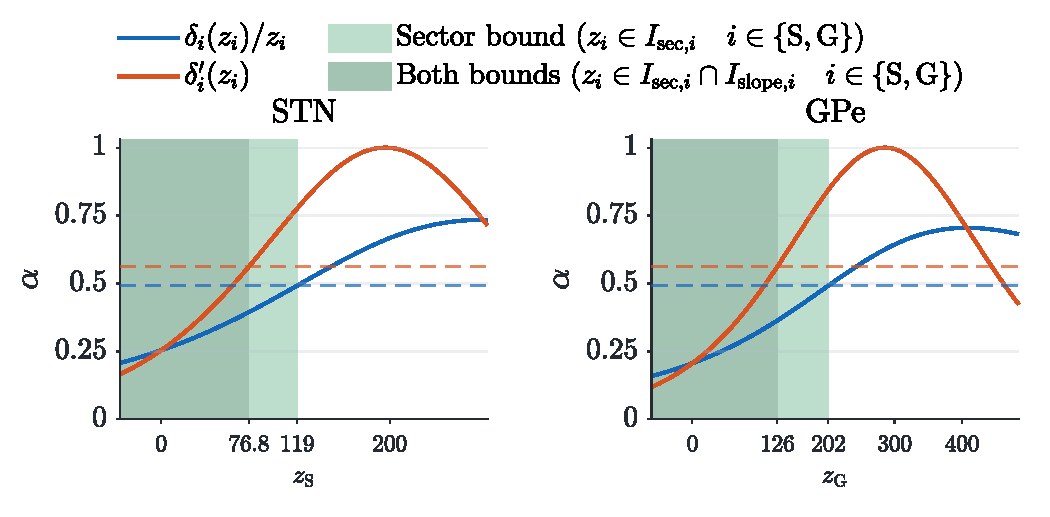
\includegraphics[width=\linewidth]{Figures/stn_gpe_admissible_trajectories.pdf}
\caption{Sector and slope bounds for the shifted STN and GPe nonlinearities. Dashed lines mark the maximum certified bounds $0.492$ and $0.562$. Shaded regions show the corresponding admissible input ranges. The larger Zames--Falb bound does not imply a wider trajectory interval because the sector and slope constraints have different geometry.}
\label{fig:admissible}
\end{figure}

Figure~\ref{fig:admissible} compares the two admissible regions. Although the Zames--Falb IQC certifies a larger scalar bound, its associated admissible input interval is smaller for this operating point. Thus the bound values alone do not rank the practical trajectory ranges; the shape of each nonlinear constraint matters.

\subsection{Closed-loop simulation}

We simulate the shifted nonlinear model with the controller synthesized using the static sector IQC at $\alpha_{\mathrm{sec}}^\star=0.492$. The initial deviations are $x_{\Srate}(0)=x_{\Grate}(0)=0$. To perturb the uncertain interconnection, we inject the pulse
\begin{equation}
d(t)=\begin{cases}
\bmat{10\\-10}\sin^2\!\left(\dfrac{\pi(t-0.10)}{0.04}\right),&0.10\leq t\leq0.14,\\
0,&\text{otherwise}.
\end{cases}
\label{eq:pulse}
\end{equation}
The sector-admissible input limits are $z_{\Srate}^{\max}=119.09$ and $z_{\Grate}^{\max}=201.85$. Figure~\ref{fig:simulation} shows that both inputs remain within their certified ranges for this perturbation, and the firing-rate deviations return toward the equilibrium.

\begin{figure}[t]
\centering
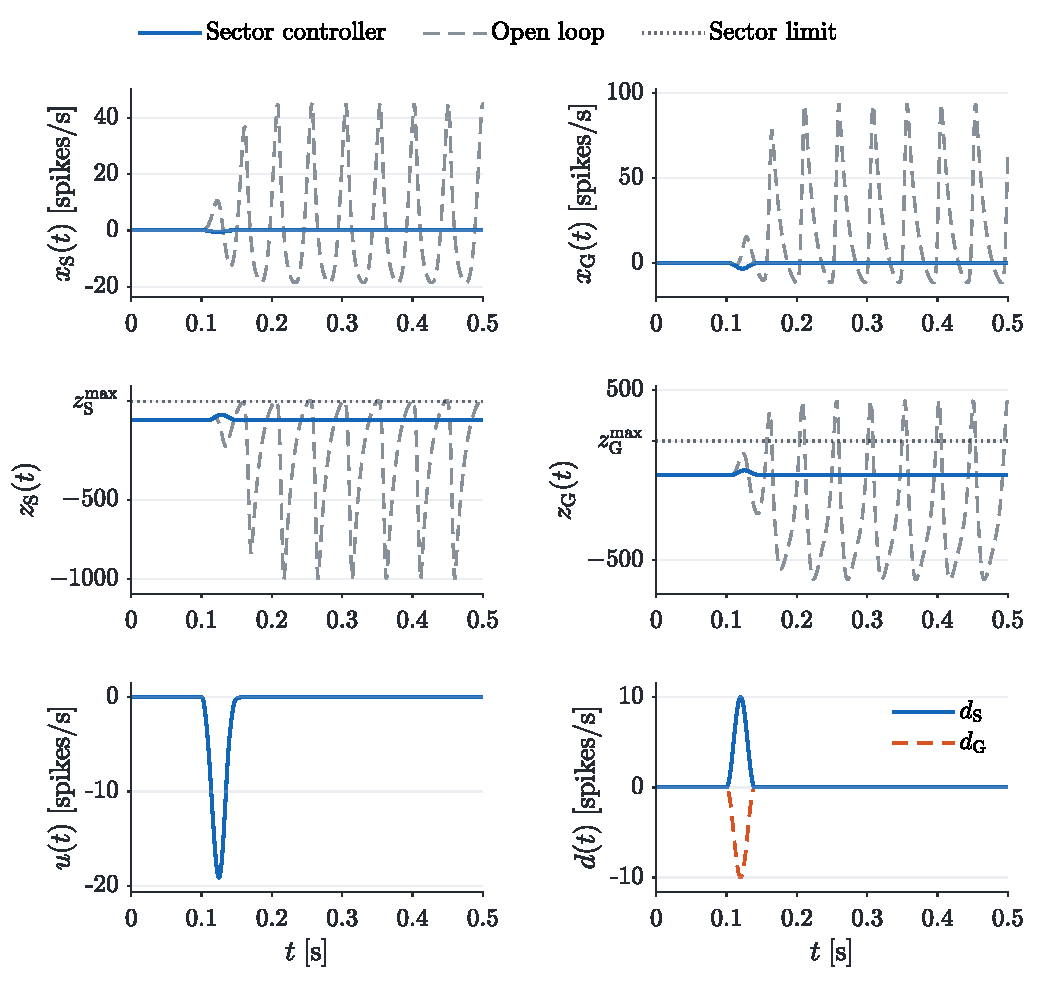
\includegraphics[width=\linewidth]{Figures/stn_gpe_sector_trajectories.pdf}
\caption{Closed-loop response of the shifted nonlinear STN--GPe model under the pulse disturbance~\eqref{eq:pulse}. Top: firing-rate deviations. Middle: nonlinearity inputs and sector-admissible limits. Bottom: control effort and injected disturbance. The displayed trajectory remains within the sector-certified input ranges.}
\label{fig:simulation}
\end{figure}

\section{Discussion}

The case study illustrates how transport-equation representations make fixed transmission delays compatible with PIE robust-control tools. The static sector IQC gives a direct trajectory-dependent certificate, while the dynamic Zames--Falb IQC uses monotonicity and slope information. In this example the dynamic multiplier certifies the larger scalar slope bound, but its admissible input interval is not uniformly larger. This distinction matters when interpreting IQC bounds for a nonlinear population model.

The conclusions are limited to the stated STN--GPe equations, parameter set, equilibrium, uncertainty descriptions, and computed certificates. The simulation illustrates one perturbed trajectory; robust stability follows from the synthesis certificate under its assumptions, not from the simulation alone. The model-based results do not establish physiological efficacy or experimental closed-loop performance. Future work can examine parameter uncertainty, alternative neural population models, measurement constraints, and experimentally grounded controller objectives.

\section{Conclusion}

We studied robust closed-loop control of delayed neural activity in a firing-rate model of the STN--GPe network. A transport-PDE representation enabled dual-IQC LPI synthesis for both static sector and dynamic Zames--Falb descriptions of the nonlinearities. For the selected equilibrium, the method certified bounds of $0.492$ and $0.562$, respectively, and the sector-based simulation remained within the certified input range under a pulse perturbation. The results provide a reproducible model-based example of robust control for delayed neural population dynamics.

\bibliography{references}

\end{document}
